\uuid{zL1k}
\niveau{PCSI}
\module{Analyse}
\chapitre{Généralités sur les nombres réels}
\sousChapitre{\'Equations et inéquations}
\duree{10}
\difficulte{1}
\auteur{Antoine Crouzet}
\datecreate{01/12/2024}
\titre{Inéquation}
\contenu{
\question{Résoudre l'inéquation : \[ \frac{(x+1)(x-2)}{2x+1} > 0 \]}
\reponse{\begin{align*}
On dresse le tableau de signes sur $\R \backslash \left \{ -\frac{1}{2}\right \}$, $-\frac{1}{2}$ étant une valeur interdite :
\begin{center}
\begin{tikzpicture}
   \tkzTabInit[espcl=1.5,lgt = 3]{$x$ / 0.9 , $x+1$ / 0.7, $x-2$ / 0.7,  $2x+1$ / 0.7, $\frac{(x+1)(x-2)}{2x+1}$ / 0.7}{$-\infty$, $-1$, $-\frac{1}{2}$, $2$, $+\infty$}
   \tkzTabLine{,-,z,+,,+,,+,}
   \tkzTabLine{,-,,-,,-,z,+,}
   \tkzTabLine{,-,,-,z,+,,+,}
   \tkzTabLine{,-,z,+,d,-,z,+,}
\end{tikzpicture}
\end{center}
On en déduit que l'ensemble des solutions de l'inéquation est \[ \boxed{\mathcal{S}=\left ]-1, -\frac12\right[ \cup \interoo{2 +\infty}}\]
\end{align*}}
}
